\documentclass[11pt,letterpaper]{article}
\usepackage[utf8]{inputenc}
\usepackage{authoraftertitle}
\usepackage[left=3cm,right=3cm,top=3cm,bottom=3cm]{geometry}

\usepackage{hyperref}

\usepackage{amsmath}
\usepackage{amsfonts}
\usepackage{amssymb}
\usepackage{fourier}
\usepackage{cancel}
\usepackage{mathtools}

\usepackage{graphicx}
\usepackage{float}

\usepackage{enumitem}
\usepackage{fancyhdr}

\usepackage{circuitikz}

\usepackage{minted}
\usemintedstyle{colorful}

\author{YOUR NAME HERE}
\newcommand{\course}{COURSE CODE}
\newcommand{\id}{STUDENT ID}
\newcommand{\assignment}{Assignment \#}
\newcommand{\soln}{\textbf{Solution}}

\setlength{\parindent}{0em}
\setlength{\parskip}{1em}

\pagestyle{fancy}
\lhead{\MyAuthor}
\rhead{\id}
\rfoot{\course{} \assignment{}}
\lfoot{\today}

\begin{document}
\section*{\course{} \assignment{}}

\subsection*{Question Title}

Question Description
\begin{enumerate}[label=\alph*.]
  \item This is a multi part question

    \soln{}

    I like to put my solutions inline

  \item This is another part 
\end{enumerate}

\soln{}

But a solution can also come afterwards.

This is how an equation is defined
\begin{equation}
  \boldsymbol{Ax} = \boldsymbol{b}
\end{equation}
but an equation can also be \textit{inline} like this $y = mx + b$.

\begin{figure}[H]
  \centering
  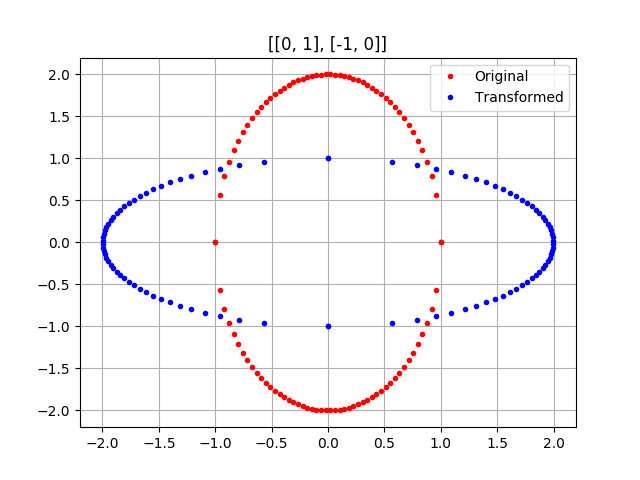
\includegraphics[scale=0.5]{photos/my_img}
  \caption{Photos can also be added like this}\label{fig:img}
\end{figure}

Images can be referenced using~\ref{fig:img}.

\begin{itemize}
  \item Items

  \item are declared like this.
\end{itemize}

Here is a circuit
\begin{figure}[H]
\centering
\begin{circuitikz}[american voltages]
\draw
(0,0)
  to[open, *-*, v^<=$v_i$]
(0,2) 
  to[L, l=$j \omega 250\ \text{mH}$]
(2,2)
  to[R, l^=$1.5\ \text{k}\Omega$]
(2,0)

(2,2)
  to[short]
(4,2)
  to[open, *-*, v^=$v_o$]
(4,0)
  to[short]
(0,0)
;
\end{circuitikz}
\end{figure}

Here is some code
\begin{minted}{python}
def my_func(arg):
    """A nice docstring."""
    return arg + 1
\end{minted}
I usually do inline code like \texttt{this} but there are other options.

Here is a table~\ref{tbl:table}. I typically generate these with
\url{http://www.tablesgenerator.com/}
\begin{table}[H]
\centering
\caption{This is a table.}\label{tbl:table}
\begin{tabular}{|l|l|l|}
\hline
\textbf{Sample} & \textbf{Value} & \textbf{Other Value} \\ \hline
A               & 7              & 87                   \\ \hline
B               & 3              & 1                    \\ \hline
\end{tabular}
\end{table}
                                                          
\end{document}                                            
